%%%%%%%%%%%%%%%%%%%%%%%%%%%%%%%%%%%%%%%%%%%%
%%% MEDICINALS
%%%%%%%%%%%%%%%%%%%%%%%%%%%%%%%%%%%%%%%%%%%%

\mysection{Medicinals}{research-medicinals}

Medicinals allow you to heal the more permanent ailments that might be afflicting the other members of your Band.   To practice your craft, the Settlement where you're taking the Vacation must have a Sanitarium and/or Library present (see the Core Rules).  Medicinals require no coin, but you can make a donation to the Sanitarium or Library if you'd like (up 200 coins of the appropriate type per Research spent) in order to convert coin to Glory.

\mysubsection{Cure Disease}{research-medicinals-cure-disease}

\example{
   2 Research per Disease
}

You can cure any disease currently infecting your Ally.  Each disease requires 2 Research.

  \begin{center}
  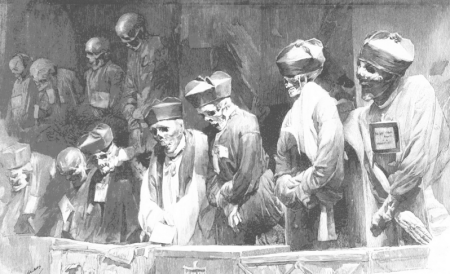
\includegraphics[scale=.5]{Medicinals}
  \end{center}

\cbreak

\mysubsection{Rehab}{research-medicinals-rehab}

\example{
   6 - (\MAX Overdose) Research
}


You can cure someone's addiction to Narcotics.  The cost is a number of Research equal to 6 minus the \MAX Overdose rating of the narcotic in question (for example, Pipeweed has a \MAX Overdose of 4, so it would require 2 Research; Yellow Opium has a \MAX Overdose of 1, so it would require 5 Research).  The recovering addict will have the permanent effect listed under Recovery (see the Core Rules).

\mysubsection{Serious Wounds}{research-medicinals-wounds}

\example{
   2 Research per Wound
}


Through your gentle ministrations over the course of a Vacation, you heal a patient's Beating, Madness, or Life Drain.  The cost is 2 Research per Wound mended.

